% A simple fault tree
% Author: Zhang Long, Mail: zhangloong[at]gmail.com
%\def\pgfsysdriver{pgfsys-dvipdfm.def}
\documentclass{minimal}
\usepackage{tikz}
\usetikzlibrary{shapes.gates.logic.US,trees,positioning,arrows}
\begin{document}
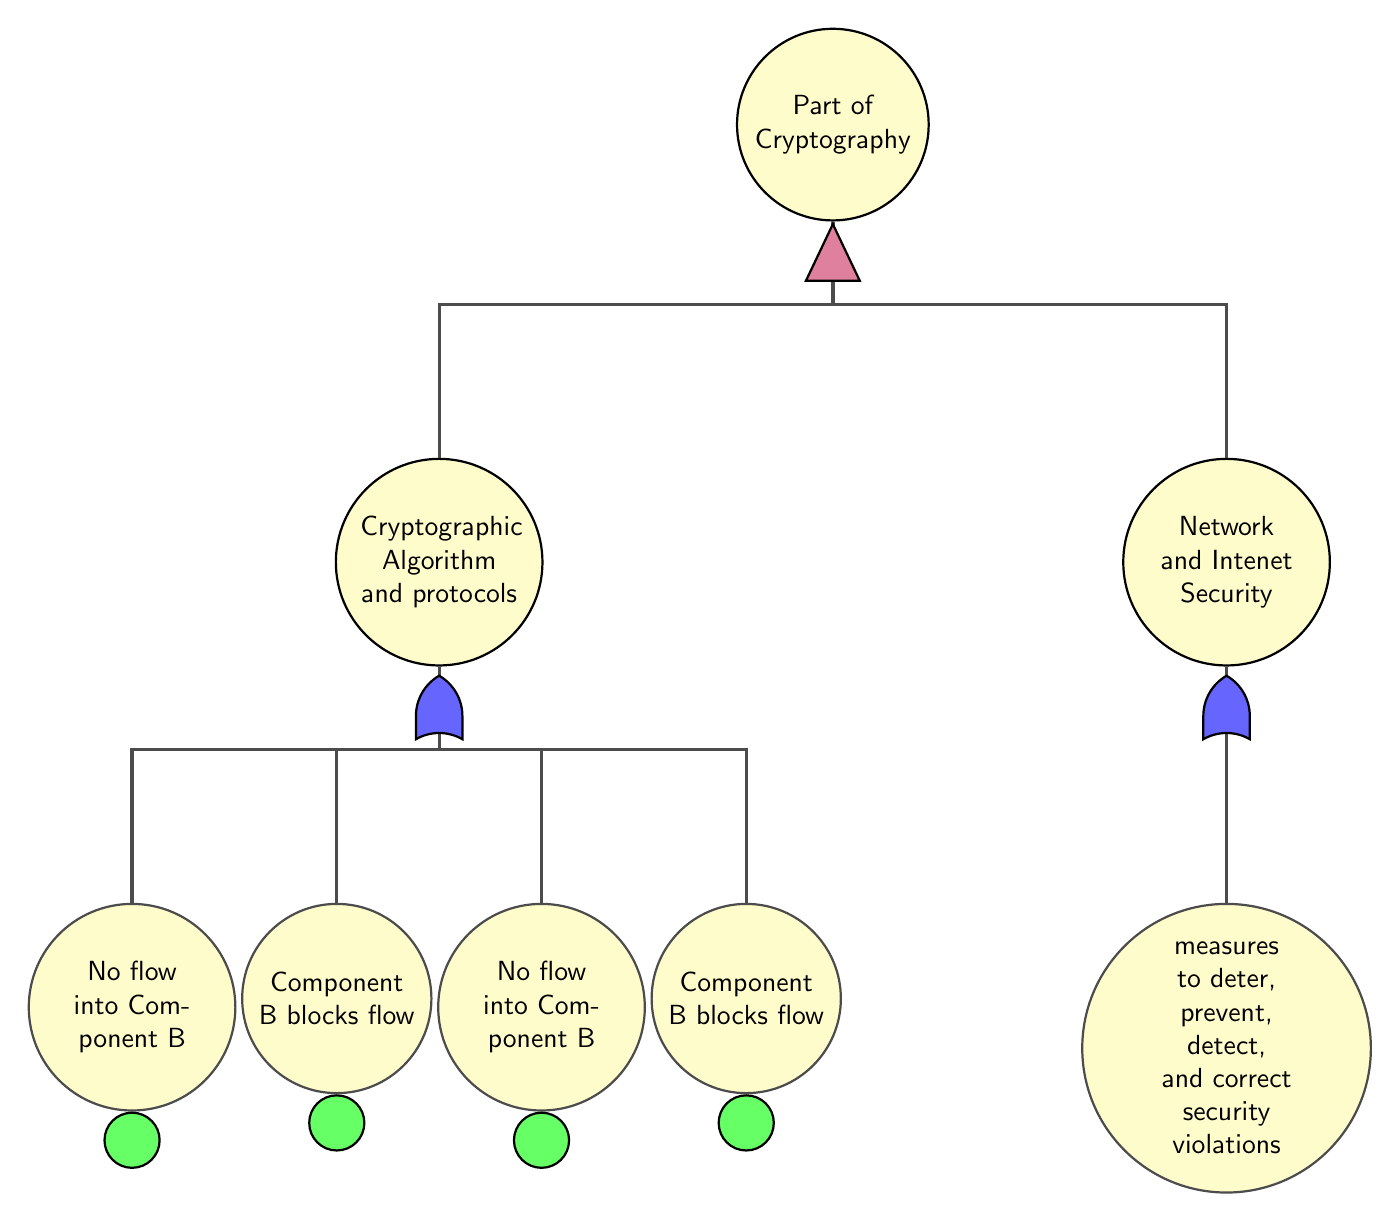
\begin{tikzpicture}[
% Gates and symbols style
    and/.style={and gate US,thick,draw,fill=red!60,rotate=90,
		anchor=east,xshift=-1mm},
    or/.style={or gate US,thick,draw,fill=blue!60,rotate=90,
		anchor=east,xshift=-1mm},
    be/.style={circle,thick,draw,fill=green!60,anchor=north,
		minimum width=0.7cm},
    tr/.style={buffer gate US,thick,draw,fill=purple!50,rotate=90,
		anchor=east,minimum width=0.8cm},
% Label style
    label distance=3mm,
    every label/.style={blue},
% Event style
    event/.style={circle,thick,draw,fill=yellow!20,text width=2cm,
		text centered,font=\sffamily,anchor=north},
% Children and edges style
    edge from parent/.style={very thick,draw=black!70},
    edge from parent path={(\tikzparentnode.south) -- ++(0,-1.05cm)
			-| (\tikzchildnode.north)},
    level 1/.style={sibling distance=10cm,level distance=3cm,
			growth parent anchor=south,nodes=event},
    level 2/.style={sibling distance=2.6cm},
    level 3/.style={sibling distance=6cm},
    level 4/.style={sibling distance=3cm}
%%  For compatability with PGF CVS add the absolute option:
%   absolute
    ]
%% Draw events and edges
    \node (g1) [event] {Part of Cryptography}
		child{node (a1) {Cryptographic Algorithm and protocols}
	     	child {node (b11) {No flow into Component B}}
	     	child {node (b12) {Component B blocks flow}}
	     	child {node (b13) {No flow into Component B}}
			child {node (b14) {Component B blocks flow}}
		}
	 	child{node (a2) {Network and Intenet Security}
	 		child {node(b21){measures to deter, prevent,
	 			detect, and correct security violations}}
 		}
	 ;
	\node [tr]	at (g1.south){};
	\node [or]	at (a1.south){};
	\node [or]	at (a2.south){};
	\node [be]	at (b11.south){};
	\node [be]	at (b12.south){};
	\node [be]	at (b13.south){};
	\node [be]	at (b14.south){};

\end{tikzpicture}
\end{document}